\chapter{Babbage-Golic time-memory tradeoff}
\label{chap:bgtmto}
\indent \textbf{\textit{Summary.}} In this chapter, we introduce time-memory tradeoff attacks on stream ciphers using the Babbage-Golic attack. Two broad scenarios are considered for the attacks: first, in which a long keystream is available to the attacker, and second, in which several short keystreams are available. Further, the first attack is divided into two categories depending on the precomputation phase in the attacks: one with random while the other with non-random precomputation. All these scenarios are implemented in the C language and the results obtained on running these attacks are presented. 

\section{Babbage-Golic attack}
\label{sec:bg-keystream-attack}

Time-memory tradeoff attacks on stream ciphers are relatively new than those on block ciphers. The first TMTO attack was conceptualized in \cite{hellman1980ctm} by Hellman on the block cipher DES in the year 1980. In contrast, the first and the simplest TMTO attack on stream ciphers was published by Babbage \cite{babbage} and Golic \cite{golic}, independent of each other in 1995 and 1997 respectively. We call this attack on stream ciphers as the BG attack. We explain the original BG attack and a variant of it in the sections \ref{sec:bg-r} and \ref{sec:bg-nr}.

\subsection{Attack with random precomputation}
\label{sec:bg-r}

As discussed in section \ref{sec:psrg}, PRSG generates a long keystream using a short secret key, to which the bits of the plaintext are \emph{xor}'ed giving the ciphertext bits. In this way, a stream cipher is produced. A simple external model of the PRSG taken from \cite{babbage} is shown in figure \ref{fig:psrg-model}. The initial state of the PRSG is $S_0$, which is derived using the secret key and other initialization parameters. The consequent states are indicated by $S_i$. The right arrow represents the update function while the downward arrow represents the output function. We assume that the PRSG incorporates an LFSR having the maximal period of $2^{n} - 1$.

\begin{figure}[h]
	\centering
	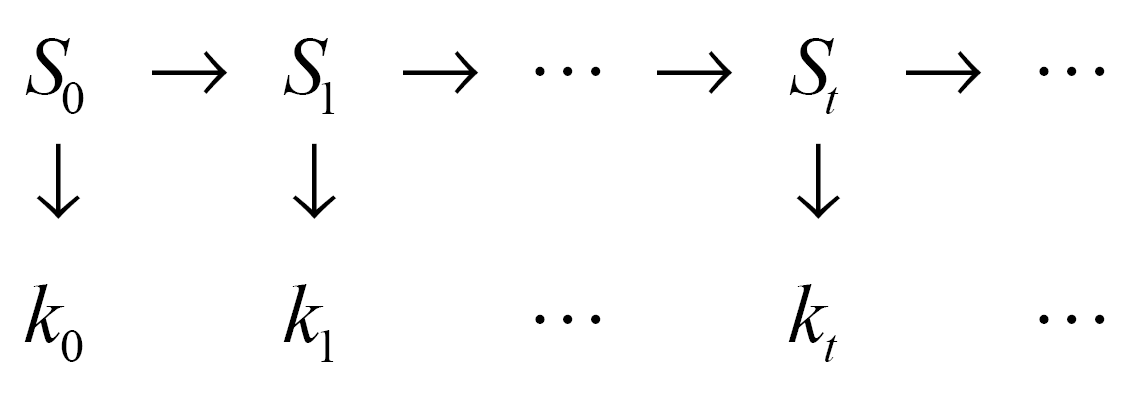
\includegraphics[width=3in]{./figures/prsgmodel.png}
	\caption{External model of a PRSG \cite{babbage}}	
	\label{fig:psrg-model}
\end{figure}

The keystream bits are represented by $k_0$, $k_1$, $\ldots$ , $k_{t}$. The goal of the attacker is to find at least one internal state which occurs while the keystream is generated, with the knowledge of the keystream (or part of it). The attacker could then move the PRSG forward to generate more keystream, in case limited keystream is known. Or the found internal state could be used to run the PRSG backwards and find the initial state. From the initial state, finding the key is not a difficult task if the cipher algorithm and initialization parameters are known. \\

\noindent \textit{\textbf{Prefix of the output sequence of states.}} If the current state of the PRSG is $S_r$, then an infinite output sequence\footnote{infinite but repeating sequence} can be generated by clocking the PRSG from that state. The sequence of first $p$ bits of this output sequence is called \textit{prefix} of state $S_r$ and represented by the bits $k_r$, $k_{r+1}$, $\ldots$ , $k_{r+p-1}$. The importance of this is that by using a prefix from the keystream, we intend to identify the current internal state of the PRSG.

A prefix is usually unique to the state if $p$ is greater than or equal to $n$ \cite{biryukov2000rtc}. If the size of the prefix is less than $n$, then there would be many states which generate the same prefix. 

For example, consider state size of 48 bits (as in HiTag2) and prefix of length 32 bits. The size of the state space and the prefix space are $2^{48}$ and $2^{32}$ respectively. Considering an equal (hence ideal) allocation of states to prefixes, every $2^{16}$ states would generate the same prefix. By increasing the prefix length, the probability of the prefix being unique to the state increases. If the prefix length is increased to 48 bits which is also the state size, then ideally every state generates a different prefix. An advantage of this property is taken in the BG attack. 

Later, as we shall see from experimental results, 48 bits of prefix are not sufficient for HiTag2 while 56 bits are good. This is due to the fact that HiTag2 uses a non-linear output function which results in some prefixes not occurring at all, while some occurring with more probability \cite{erik-discussions}\cite{email-karsten}.\\

\noindent \textit{\textbf{The attack.}} There are two phases in every TMTO attack: the precomputation phase and the attack phase. During precomputation, the attacker randomly selects $n_1$ states out of the $2^n - 1$ possible PRSG states. For each of these states, the prefix of size $p$ = $n$ is computed, and the (prefix, state) pair stored in memory. The data structure used for storing the pairs is hashtable, which is introduced in section \ref{sec:hash-tables}. Prefix is used as the hashkey while the state is used as the hashvalue in a pair.

During the attack phase, the attacker is assumed to know some part of the initial keystream. In practice, the attacker knows the ciphertext. Assuming that the attacker has knowledge of the plaintext by some means, the keystream bits can be calculated as, $k_i$ = $p_i \oplus c_i$. 

The attacker then selects overlapping subsequences of size $p$ from the keystream. The first subsequence would be $k_0$, $k_1$, $\ldots$ , $k_{p-1}$, the second subsequence would be $k_1$, $k_2$, $\ldots$ , $k_{p}$ and so on. Each of these subsequences is then matched with the prefixes stored in the hash table. If there is a match, the current state is retrieved from the matched (prefix, state) pair. Say that the $i$'th subsequence from the keystream is found in the hashtable. Then the following two actions are performed by the attacker.
\begin{itemize}
\item The current state is reversed $i$ times to get the initial state of the cipher. 
\item Once the initial state is known, the secret key can be retrieved if the other initialization parameters are known.
\end{itemize} 
Reversing the internal state can be performed since the update function of HiTag2 is known. In addition, in HiTag2, the serial ID and the IV are used in initialization process, in addition to the key. The serial ID is specific to the car key, while the IV is changed during every protocol run, and both can be easily known to the attacker. So further getting the key from the initial state is not a difficult task. 

In the HiTag2 library, the functions which implement these two actions are \textit{hitag2\_prev\_state} and \textit{hitag2\_find\_key}. The function \textit{hitag2\_prev\_state} basically performs the reverse action of the update function and is called $i$ times to revert to the initial state. The \textit{hitag2\_find\_key} function returns the key if provided with this initial state and the known serial ID and IV.

It is important to note that these last two actions are common to all attacks on stream ciphers discussed in this thesis (except for the attack discussed in section \ref{sec:bg-tags-attack}). So for these attacks, we shall only concentrate on how the current state is found from the known keystream. This is primarily the goal in attacks on stream ciphers: to find an internal state.\\

\noindent \textit{\textbf{Parameters in the attack.}} We introduce certain important parameters here \cite{biryukov2000ctm} which are used to represent a general tradeoff attack like the BG attack. These parameters would help us in understanding where an ideal line be drawn between memory and time requirements during the precomputation and attack phases, so that the attack is feasible (say, with respect to a personal computer). These are general parameters and are used for describing all attacks in the thesis. 

\begin{enumerate}
\item \emph{M} represents the order of memory size required for hashtable.
\item \emph{P} represents the order of time required for the precomputation phase.
\item \emph{T} represents the order of time required for the attack phase.
\item \emph{D} represents the order of prefixes available during the attack phase.
\end{enumerate}

In the paper \cite{biryukov2000ctm}, these parameters are introduced without the term \mbox{`order'}. We stress here that the parameters do not represent the actual time and memory values in seconds and bytes, but they represent the order of the magnitude of these values.\\

\noindent \textit{\textbf{Tradeoff equation.}} Let us assume that $n_1$ states are selected during the precomputation phase, while during the attack phase the PRSG traverses through $n_2$ states. $M$ is equal to $n_1$, since the size of the hashtable depends on the number of states stored. Similarly, the time to prepare the hashtable is proportional to $n_1$, hence the order of this time, or $P$, is $n_1$. As a result, $M$ = $P$ = $n_1$.

Since $n_2$ states are traversed while generating the keystream, it is desirable that the prefix of all these states be available in order to attempt matching $n_2$ prefixes in the hashtable. If prefix of length $n$ is used for every state, then the length of the keystream should be at least $(n_2 + n - 1)$ bits. In such a case, since $n_2$ prefixes are searched in the hashtable, the order of time for the attack is $T$ = $n_2$. Similarly, if we consider one prefix as datum, then the order of data available is $n_2$, thus $D$ = $T$ = $n_2$.

Now we have a clear setting for applying equation \ref{eq:bday-paradox2} of the birthday paradox. In a set of $2^n$ states (ignoring that something like the trivial state exists at all), $n_1$ states are selected in precomputation and $n_2$ are selected during the attack. According to the variant of the birthday paradox we then have the following condition,
\begin{align}
& n_1 \times n_2 \geq 2^n\\
\label{eq:bgattack-tradeoff} & M \times T \geq 2^n
\end{align}
The equation \ref{eq:bgattack-tradeoff} is the condition for a successful attack. Though the condition is probabilistic, the probability of a match is very high if the parameters of $M$ and $T$ are wisely chosen according to this equation.

\subsection{Attack with non-random precomputation}
\label{sec:bg-nr}

The precomputation in BG attack is done by randomly generating states of $n$ bits, and then computing their prefix. The other way of performing the precomputation is by selecting states through a deterministic algorithm. Let's say the internal state of a stream cipher runs through all $2^n - 1$ possible states, which is represented by a huge cycle of states. If we select states at a fixed distance $d$ from each other during precomputation, we can be sure that there would be a match if the attack phase has a time order also of $d$ \cite{erik-discussions}. This represents the core idea behind non-random precomputation and is explained in detail in the further paragraphs. The HiTag2 cipher is well suited for this attack, since it's internal state runs through the longest possible cycle of $2^{48} - 1$ states. The attack phase remains the same as in case of randomly selected precomputation states.\\

\noindent \textit{\textbf{Non-random precomputation phase.}} During the precomputation phase, the selection of states is not done at random. An initial state is selected at random ($S_{initial}$), while the remaining states are derived using this state. The prefix for $S_{initial}$ is first computed and the (prefix, state) pair stored in the hash table. The next state is derived using a \emph{state transition function} (construction of which is explained in detail later), which returns the state $d$ states ahead of the current state, represented by $S_{initial+d}$. Similarly, the prefix for $S_{initial+d}$ is computed and the (prefix, state) pair stored in the hash table. The process is repeated giving us the sequence of states: $S_{initial}$, $S_{initial+d}$, $S_{initial+2d}$ and so on. 

The number of states required in the hashtable is $M$. Hence, the distance between each state should be $d$ = $2^n/M \Rightarrow M = 2^n/d$. $P$ would be the same as $M$ in this case as well, and we have the relation $M$ = $P$ = $2^n/d$.\\

\noindent \textit{\textbf{Attack phase.}} The initial state which generated the available keystream is unknown to the attacker. The attacker selects subsequences from the keystream and matches them with the prefixes stored in the hashtable. Now, in order to guarantee that atleast one prefix would match, it is sufficient to have $d$ states during the attack. This is ensured if keystream of length ($d + n - 1$) bits is available to the attacker. Since any two states in the hashtable are $d$ states apart, in the worst case if $d$ unknown states are traversed during the attack, atleast one state is bound to match. Consequently, we have the requirement that $D$ = $d$, which also means $T$ = $d$ as the time of the attack depends on the length of the available keystream.\\

\noindent \textit{\textbf{Tradeoff equation.}} From the above analysis, we have $M = 2^n/T$ which leads to the following tradeoff equation.
\begin{align}
\label{eq:tmto-non-random} M \times T = 2^n
\end{align}
Using this equation, the time and memory for the attack can be varied. It is interesting to compare this equation with the equation for the attack with random precomputation. The latter was based on the birthday paradox, and hence the chances of finding a match are always close to 100\%, but not exactly 100\%. The greater the value $M \times T$ as compared to $2^n$, the more is the chance of success. In case of non-random precomputation, the chances of a match are exactly 100\% if $M$ and $T$ are selected according to equation \ref{eq:tmto-non-random}.\\

\noindent \textit{\textbf{State transition function.}} As mentioned above, the \emph{state transition function} is used in the precomputation phase for computing a non-adjacent state directly from the current state. If we use the update function in order compute the state $d$ distance ahead, the function would be called $d$ times and thus take a total computation time of an order $d$. If this has to be repeated in order to cover the entire cycle of states, the precomputation time would be of the order of $2^n$. There is no doubt that this is not feasible; otherwise a brute force attack with $2^n$ computations would not have been a bad idea! 

Hence, a function is required which computes the $d$'th state in constant time, thus keeping the precomputation time order the same as $2^{n}/d$. We refer to this function as the state transition function and its design is discussed next. 

An update function can be represented by a binary matrix $U$ \cite{trappe2005icc}\cite{erik-discussions}. This matrix on multiplication with the binary matrix representation of the current state gives the binary matrix of the adjacent state. If the current state of the LFSR is $S_{current}$, then the next state $S_{next}$ can be computed by the matrix multiplication shown below.
\begin{center}
$U . S_{current}$ = $S_{next}$\\
\end{center}
This is represented in the matrix notation as follows.
\begin{center}
$U.$
$\begin{bmatrix}
s_{n} \\
s_{n-1} \\
\vdots \\
s_{1} \\
s_{0}
\end{bmatrix}$ = 
$\begin{bmatrix}
s_{new} \\
s_{n} \\
\vdots \\
s_{2} \\
s_{1}
\end{bmatrix}$
\end{center}

\begin{figure}[h!]
	\centering
	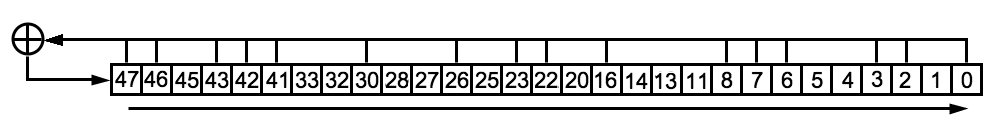
\includegraphics[width=5in]{./figures/hitag2-update-function.png}
	\caption{Update function $U$ for HiTag2}	
	\label{fig:hitag2-update-function}
\end{figure}

The topmost row of $U$ represents the tap sequence and contains a `1' at positions representing the tap bits, and a `0' otherwise. This row is multiplied with the current state to give the new bit (the leftmost bit) of the LFSR. The remaining rows of $U$ are setup in such a way that the remaining bits of the LFSR are shifted one place rightwards, as indicated by the update function of HiTag2 in figure \ref{fig:hitag2-update-function}. 

It must be noted that the indexing in the matrix is the same as that in the LFSR. Thus, the leftmost bit in the topmost row of $U$ represents the $48^{th}$ bit of the LFSR, and the rightmost bit represents the $1^{st}$ bit. In addition, in the state matrices $S_{current}$ and $S_{next}$, the topmost bit represents the $48^{th}$ bit of LFSR and the bottommost bit represents the $1^{st}$ bit. The matrix $U$ for HiTag2 is shown in figure \ref{fig:hitag2-transition-matrix} as an example.

\begin{figure}[h!]
	\centering
	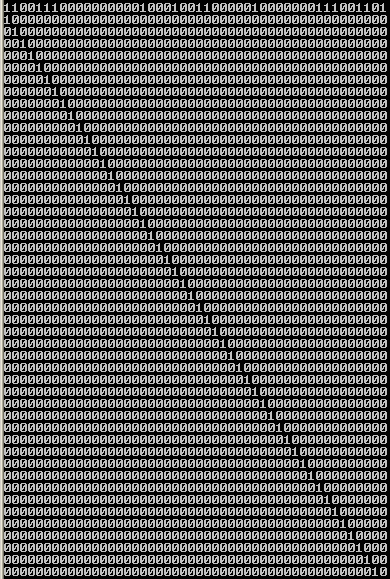
\includegraphics[width=3.5in]{./figures/hitag2-transition-matrix.png}
	\caption{Update function matrix $U$ for HiTag2}	
	\label{fig:hitag2-transition-matrix}
\end{figure}

The connection between the tap sequence of the HiTag2 LFSR and the topmost row of $U$ is easy to see from these two figures. 

Matrix multiplication of two binary matrix rows is done by first performing a bitwise boolean \emph{and} operation (denoted by \&) and then an \emph{xor} of the resulting bits. In notation, if we have two rows $r_1$ and $r_2$ of size $n$ represented by,
\begin{center}
$r_1$ = $r_{11} r_{12} \ldots r_{1n}$\\
$r_2$ = $r_{21} r_{22} \ldots r_{2n}$
\end{center}
then their multiplication is done as follows,
\begin{center}
$r_1 \times r_2$ = $(r_{11} \& r_{21}) \oplus (r_{12} \& r_{22}) \oplus \ldots \oplus (r_{1n} \& r_{2n})$
\end{center}
To compute the state occurring $d$ states after the current state, we perform the following matrix multiplication,
\begin{center}
$S_{current + d}$ = $\underbrace{U . U . U \dots U}_{d} . S_{current}$\\
\end{center}
\begin{align}
\label{eq:matrix-mult-dtimes} S_{current + d} = U^d . S_{current}
\end{align}
From \cite{erik-discussions}, there is an efficient solution for computing the states. Instead of performing matrix multiplication of $U$ $d$ times, a repeated square of the result can be performed. The square of $U$ is first computed giving $U^2$. This is squared to compute $U^4$, which is again squared to compute $U^8$, and so on. Assuming $\log_2{d}$ to be a positive integer, the squaring is repeated for $\log_2{d}$ number of times, as shown below.
\begin{align}
\label{eq:matrix-mult-logdtimes} S_{current + d} = \underbrace{(((U^2)^2) \dotsc )^2}_{\log_2{d}} . S_{current}
\end{align}
Both the equations \ref{eq:matrix-mult-dtimes} and \ref{eq:matrix-mult-logdtimes} are equivalent. Computing each state by using equation \ref{eq:matrix-mult-logdtimes} would take $\log_2{d}$ multiplications, and thus the entire precomputation phase would take $M \times \log_2{d}$ matrix multiplications. This is much efficient than the number of computations required in performing the precomputation using equation \ref{eq:matrix-mult-dtimes}. Hence equation \ref{eq:matrix-mult-logdtimes} is used in the precomputation phase of this attack.

We then represent the state transition matrix by $A$ such that,
\begin{align}
\label{eq:state-trans-matrix} A = \underbrace{(((U^2)^2) \dotsc )^2}_{\log_2{d}}
\end{align}
The matrix $A$ is computed once during the precomputation phase, and then used in computing the required states as follows,
\begin{align*}
S_{current + d} &= A . S_{current}\\
S_{current + 2d} &= A . S_{current + d}\\
&\vdots
\end{align*}
and so on, to compute $M$ states for the entire precomputation phase.

\subsection{Implementation and results}
\label{sec:keystream-attack-impl}

Both versions of the BG attack differ in the respective precomputation phase. The attack phase proceeds in the same way for random or non-random precomputation. Ofcourse, the probability of finding the key varies in both the attacks. The module implemented to carry out the complete attack performs the following tasks in sequence,
\begin{enumerate}
\item If the precomputation phase is non-random, the matrix $A$ of the state transition function is computed, otherwise it is not. To compute the state transition matrix, the update matrix is first initialized with the tap bits of the LFSR used in HiTag2 and then squared recursively, as discussed above.
\item The keystream for the attack is made available. A secret key of size $48$ bits is chosen and used in initializing the LFSR along with the serial ID and an IV. Starting with this initial state, the stream cipher is run and keystream of desired length produced and stored in memory. The length of the keystream is defined in terms of the parameter $D$ for the attack.
\item A hashtable of size $M$ is created. If the precomputation phase is non-random, the state transition matrix is used in computing subsequent states which are stored in the hashtable. Else, states are randomly chosen and stored. $P$ defines the number of times a new state is computed and $M$ defines the number of times a computed state is stored in hashtable. As we can see, in this case every time a new state is computed, it is stored in the hashtable, hence $P$ and $M$ are the same. We shall see in later attacks that $P$ and $M$ can be different depending on the algorithm for the precomputation phase. 
\item Lastly, the attack is started. Overlapping subsequences of the prepared keystream are selected and matched with the prefixes in the hashtable. The duration of the attack depends on the number of subsequences that are available, which is $D$. And thus, in this case we have $T$ = $D$. In some later attacks we shall see that this does not hold. 
\end{enumerate}

% a note about the reversing of keys. little bit of implementation details. (or to mention this in the hitag2 section?)

% a note on random function chosen? %
A random function is required to select states for the hashtable in the random precomputation phase. The $rand()$ function provided by C language library is not a cryptographically strong function, but it is good enough for the purpose of preparing states. We implemented a C program to check the period of the output of the $rand()$ function. Following are the observations made from running the program on Solaris machine.

\begin{enumerate}
\item The output of the $rand()$ function is 16 bits on the machine we used\footnote{On a different machine, we found the output to be 32 bits of length}. This is greatly insufficient for our purpose, since we require random numbers of length 48 bits.
\item If a modular 2 of the random number is taken, then the random bit sequence starts repeating after approximately $2^{17}$ bits. This was in fact our first idea for generating states i.e.~using the the modular 2 of next random number as a bit for the state, thus generating the state over 48 operations. But with this, we could clearly see that only approximately $2^{17}$ different states can be generated.
\item The 16 bit output of $rand()$ function starts repeating after $2^{31}$ random numbers. But in one period, the random numbers reoccur. This is obvious since the output has a period $2^{31}$ whereas the output space size is just $2^{16}$. So, we implemented a wrapper using $rand()$, such that the 16 bits of the output are left shifted by one bit and \textit{xor}'ed with the next output, this repeating 32 times to generate 48 bits. The code snippet for this is shown below. Here, u64 represents a 64 bit unsigned integer and u32 represents a 32 bit unsigned integer.
\begin{lstlisting}[frame=tb]
u64 get_random_2(u32 bits)
{
	u32 i = 0;
	u64 random_number = 0;
	u64 rand_out = 0;

	for(i = 0; i < bits - 16; i++)
	{
		rand_out = rand();
		random_number = 
			(random_number << 1) ^ rand_out;
	}

	return random_number;
}
\end{lstlisting}
The program for checking the period of this random number generator is given in appendix \ref{app:random-function}.
\item If we generate a 32 bit random number using this function, the period observed is $2^{27}$. Also, the period for 48 bit random numbers is $2^{26}$. We do not generate more than $2^{26}$ random states in the implementation (as seen from the values of $M$ in table \ref{tab:keystream-attack-results-key1} and \ref{tab:keystream-attack-results-key2} below), hence the wrapper function is sufficient for our purpose.
\end{enumerate}

The attack is run on a terminal on the Sun Solaris server which is shared among various users. Because of this, the computational speed used for the attacks cannot be determined precisely. Also, this causes divergence in some results from their expected values. Most of the attacks are carried in this environment. Where this is not the case, comments are explicitly made in the thesis. 

Three different keys are randomly selected for the attacks. One or more keys from these three are used in all the attack implementations. These keys are as follows.

\begin{enumerate}
\item Key $K_1$ = 0x52B49EA34972
\item Key $K_2$ = 0xD4E98D3DA2F2
\item Key $K_3$ = 0x49D2AC801F94
\end{enumerate}

We display the results for the first two keys $K_1$ and $K_2$ in tables \ref{tab:keystream-attack-results-key1} and \ref{tab:keystream-attack-results-key2} respectively. The values of $M$ and $T$ are varied for each key, for both random and non-random precomputation phase. A very important parameter in the attack is the length of the prefix. We have chosen prefix length of $48$ and $56$ bits for the keys. Prefix length lower than 48 bits would lead to greater number of false keys, while prefix length higher than 56 bits would not be any better since 56 bits prefix length is sufficient in eliminating false keys (which is also confirmed by the results). Hence these two prefix lengths are considered for the experiments. The time taken for the preparation of the hashtable and keystream, and for the attack are all given in seconds. 

\begin{table}[ht!]
\begin{center}
\begin{tabular}{|p{3cm}||c|c|c|c|c|c|c|c|c|c|}
\hline
\multicolumn{11}{|c|}{\textbf{Key $K_1$ = 0x52B49EA34972}} \\ \hline \hline
Precomputation 	& \multicolumn{5}{c|}{Random} & \multicolumn{5}{c|}{Non-random} \\ \hline
Prefix length										&	48 				&	48 				&	48 				&	48 				& 56 				&	48 				&	48				&	48 				&	56 				&	56  			\\ \hline
M																&	$2^{21}$ 	&	$2^{22}$ 	&	$2^{24}$ 	&	$2^{25}$ 	&	$2^{25}$ 	& $2^{21}$ 	&	$2^{21}$ 	&	$2^{21}$ 	&	$2^{21}$ 	& $2^{21}$	\\ \hline
T	  														&	$2^{26}$ 	&	$2^{25}$ 	&	$2^{25}$ 	&	$2^{25}$	&	$2^{25}$ 	& $2^{26}$ 	&	$2^{27}$ 	&	$2^{28}$ 	& $2^{27}$ 	& $2^{28}$	\\ \hline
Time for preparing hashtable		&	16 				&	32 				&	128				&	256				&	279 			& 88 				&	87				& 87				&	89	 			& 89				\\ \hline
Time for preparing keystream		&	6 				&	3 				&	3 				&	3 				&	3 				& 6 				&	12				& 24				&	12				& 24				\\ \hline
Time for attack									&	54 				&	28 				&	29 				&	31 				&	29 				& 56 				&	113				& 223				&	109				& 221				\\ \hline
Number of times key is found		&	0 				&	0 				&	0 				&	2 				&	2 				& 1 				&	1					& 2 				&	1 				& 2					\\ \hline
Number of false keys						&	0 				&	3 				&	4 				&	7 				&	0 				& 1  				&	2					& 2 				& 0 				& 0					\\ \hline
\end{tabular}
\end{center}
\caption{Results of TMTO keystream attack for $K_1$}
\label{tab:keystream-attack-results-key1}
\end{table}


\begin{table}[ht!]
\begin{center}
\begin{tabular}{|p{3cm}||c|c|c|c|c|c|c|c|c|}
\hline
\multicolumn{10}{|c|}{\textbf{Key $K_2$ = 0xD4E98D3DA2F2}} \\ \hline \hline
Precomputation 	& \multicolumn{4}{c|}{Random} & \multicolumn{5}{c|}{Non-random} \\ \hline
Prefix length										&	48 				&	48 				&	48 				&	56 				&	48 				&	48				&	48 				&	56 				&	56  			\\ \hline
M																&	$2^{22}$ 	&	$2^{23}$ 	&	$2^{22}$ 	&	$2^{22}$ 	&	$2^{22}$ 	&	$2^{21}$ 	&	$2^{22}$ 	&	$2^{22}$ 	& $2^{22}$	\\ \hline
T	  														&	$2^{26}$ 	&	$2^{26}$ 	&	$2^{27}$ 	&	$2^{27}$	&	$2^{25}$ 	&	$2^{26}$ 	&	$2^{26}$ 	& $2^{25}$ 	& $2^{26}$	\\ \hline
Time for preparing hashtable		&	29 				&	58 				&	30 				&	32 				&	178 			&	88				& 178				&	181 			& 181				\\ \hline
Time for preparing keystream		&	6 				&	5 				&	10 				&	11 				&	3 				&	6					& 6					&	3					& 6					\\ \hline
Time for attack									&	70 				&	72 				&	152 			&	148 			&	29 				&	53				& 57 				&	28 				& 55				\\ \hline
Number of times key is found		&	0 				&	2 				&	4 				&	4 				&	1 				&	0					& 1 				&	1 				& 1					\\ \hline
Number of false keys						&	0 				&	0 				&	1 				&	0 				&	1 				&	0					& 2 				& 0 				& 0					\\ \hline
\end{tabular}
\end{center}
\caption{Results of TMTO keystream attack for $K_2$}
\label{tab:keystream-attack-results-key2}
\end{table}


The following observations can be made from the above results. 
\begin{enumerate}
\item In column 3 of table \ref{tab:keystream-attack-results-key1}, we can see that $K_1$ is not found even once. On doubling $M$ as shown in the next column, it is seen that $K_1$ is found two times. This indicates that the random function we have in place for generating states for the hashtable does not repeat atleast until $2^{25}$ states. If the states would repeat, then for the same $T$ = $2^{25}$ the key would not have been found for $M$ = $2^{25}$. Hence it is confirmed that the random function and it's usage in the program is good.

\item In column 5 of table \ref{tab:keystream-attack-results-key2}, $K_2$ is found even though the product of $M$ and $T$ is less than $2^{48}$. It is thus clear that equation \ref{eq:tmto-non-random} just indicates the worst case relation between $M$ and $T$. Thus, if the product $M \times T$ $\geq$ $2^{48}$, we can be certain that the key would be found. If $M \times T$ $<$ $2^{48}$, then we cannot be certain. In this particular case, $K_2$ is found. But, another combination of $M$ and $T$ shown in column 6 exemplifies this conclusion as $K_2$ is not found in this case.

\item If the product $M \times T$ = $2^{48}$ for the non-random precomputation, then the correct key is found exactly once. However, if the product $M \times T$ = $2 \cdot 2^{48}$ (by doubling either of $M$ or $T$), then the correct key is found exactly two times. Also, the time between the second match and the first match of the key is precisely $T/2$. For the key $K_1$, output from the attack program for parameters in column 10 is shown below. The point to note here is the percentage of the worst case time for the two matches; they differ precisely by 50\%. 
\newpage
\begin{lstlisting}[frame=tb]
Match Found! 
Current State: eb444bbc2057  Prefix: d249629ec6a571

Percentage of the worst case time: 19.833907 I: 53241238

Found Initial State: 58c99e374972
Found Key: 52b49ea34972

Match Found! 
Current State: cf258b22b7b5  Prefix: 777609953446b2

Percentage of the worst case time: 69.833907 I: 187458966

Found Initial State: 58c99e374972
Found Key: 52b49ea34972
TIME for attack: 221
\end{lstlisting}

\item It is repeatedly seen that prefix length of 56 bits gives no false keys, while prefix length of 48 bits does give false keys. It is clear that 48 bits of prefix are not sufficient to represent a state uniquely. The number of false keys is not very high though, thus it can also be concluded that for every 48 bit prefix, the number of states giving a same prefix would not be many. 
 
\item The attack time for 48 bits prefix is generally more than the time for prefix length 56 bits, under the same $M$ and $T$. This is because false keys are generated for 48 bit prefixes, and it takes considerable time to find the initial state and then the key from the current state of the LFSR, before the attack resumes to search remaining prefixes in hashtable.

\item These are the first results of a TMTO attack so far in this thesis, and it can be clearly seen that if $M$ is around $2^{22}$ and $T$ is around $2^{28}$, HiTag2 can be broken in minutes on a personal computer. But, an important assumption here is the length of the available keystream.

\end{enumerate}

\newpage
\section{Babbage-Golic attack for short keystream}
\label{sec:bg-tags-attack}

In the previous attack, there is an assumption on the length of keystream available to the attacker. We have assumed that a long keystream is available, such that it is sufficient to cover the entire attack phase. Considering the use of HiTag2 in car keys, it is certain that such long keystream would not be available. Rather several short length keystream (for each transaction between the car and car key) would be available over some span of time. As explained in section \ref{sec:hitag2}, 32 bits of data is exchanged between the car and the car key at the start of every run of the protocol. The complete protocol is not known to us, but it is just known that these 32 bits act as authenticators between the car controller and the car key \cite{email-ruptor} \cite{hitag2-code}. This 32 bit data is known as the \emph{authenticator tag}. After authentication is successful, subsequent messages if any, are encrypted using the subsequent keystream from the cipher.

For this particular attack (which we call TMTO tags attack), we assume the availability of authenticator tags to the attacker. Also, we ignore any existence of the subsequent keystream. Hence the goal is to find the secret key by only using several authenticator tags. The difference between each of the tag lies in their initial states, which arises due to a different IV sent by the car. The secret key shared between the car and the car key is the same, and so would be the serial ID of the car key.

\subsection{TMTO tags attack}

The TMTO tags attack consists of the two TMTO phases: precomputation and attack. The precomputation phase involves selecting $M$ different initial states, computing their tags and storing the (tag, initial state)\footnote{we refer to initial state here since if a tag matches in the hashtable, the initial state is retrieved} pair in a hashtable. The time for preparing the precomputation phase is of the order of $M$, since the complexity depends on the number of tags chosen for the phase. Hence, we also have $P$ = $M$.

During the attack phase, tags are randomly generated along with their corresponding IV's (to simulate the tags collected by an attacker). These tags are then matched with the tags in the hashtable. For every tag match in the hashtable, the initial state is retrieved and the key used to initialize the cipher to that state is computed. Since each tag can be generated by approximately $2^n/2^{32}$ states, we cannot be sure that the initial state found is the one we are looking for. Hence, we continue with the matching of further tags until we find that the same key is recovered more than once. Then we can be more sure that it is the correct secret key.\\

\noindent \textit{\textbf{Tradeoff equation.}} Determining the tradeoff equation in the tags attack is discussed here. Getting to the equation is not as straightforward as in the previous attack cases, but the results are strikingly similar. The analysis has been carried out through \cite{erik-discussions}, and to our best knowledge, this analysis is not found in any literature.

Let us first consider the probability of finding a match in the hashtable. We have $M$ different states and corresponding tags in the hashtable. It cannot be guaranteed that all the tags would be different, since a tag would have more than one possible generating states (around $2^{16}$ for HiTag2 as discussed previously). In the best case, we assume that all the $M$ states generate $M$ different tags. Then, in this case, the probability of getting a tag matched in the hashtable is given by $M/2^{32}$, considering 32 bit tags. We write this probability as $P_1$, such that

\begin{center}
$P_1$ = $M/2^{32}$
\end{center}

Again, this is the best case probability and the actual probability would be less, since tags would be repeated in the hashtable. Next, we need to determine the probability that a match yields the correct initial state and thus the correct key. This can be determined in the following way: the number of different states is $2^n$ and the number of different tags is $2^{32}$. Then, the probability that the matched tag be representing the correct internal state is $2^{32}/2^n$. This probability is represented by $P_2$ such that
\begin{center}
$P_2$ = $2^{32}/2^n$
\end{center}
The overall probability of finding the correct state is given by $P$, such that
\begin{align*}
P &= P_1 \cdot P_2\\
P &= M/2^{n}
\end{align*}
This is the probability of the correct key being found when we have one tag. Hence, for the correct key to be found atleast once, the runtime of the attack phase must be of an order of atleast $2^{n}/M$ so that we have $2^{n}/M$ tags. Hence, we can say that
\begin{align}
T &\geq 2^{n}/M\\
\label{eq:tmto-tags-equation} M \cdot T &\geq 2^{n}
\end{align}
In practice, the product of $M$ and $T$ must be larger than $2^n$ for the correct key to be found once, since we considered the best case probability while calculating $P_1$. Practically, $P_1$ would be less than its value in the above equation, which would lead to a lower $P$. With lower $P$, $T$ would have to increased if we want to find the correct state. The equation for $P$ just gives us an approximate value of $M$ and $T$, and it is much probable that the attack is successful for higher values of the two parameters.

The other important issue here is that several tags would match during the attack, thus resulting in several possible keys. The correct key is expected to be found only once if $M$ and $T$ are chosen according to equation \ref{eq:tmto-tags-equation}. If the values of $M$ and $T$ are so chosen that we have $M \cdot T \geq 2 \cdot 2^{n}$, then the correct key is expected to be found atleast two times. Similarly, if we have $M \cdot T \geq 4 \cdot 2^{n}$, then we can expect to find the correct key four times, and so on. Using this idea, the correct key is determined from among all the keys derived from the matched tags. 

\subsection{Implementation and results}

The implementation module for TMTO tags attack executes the complete attack by carrying out the following tasks in sequence. 

\begin{enumerate}

\item Only the non-random precomputation phase for this attack is chosen. Hence the first step is to initialize the update function matrix and state transition matrix.
\item The hashtable is prepared. A fixed 48 bit value is used as the starting state, and equidistant states and their 32 bit prefixes are stored in the hashtable, with the prefix as the hashkey and state as the hashvalue. The size of the hashtable is $M$, and thus the distance between each state stored is fixed to $2^{48}/M$. Also, the time for preparing the hashtable is $P = M$, since each state computed during precomputation is stored in the hashtable.  
\item The required number of tags for the attack are prepared. It is assumed that the attacker captures 32 bit tags and the IV sent along with it when one run of the authentication protocol takes place between the car and the car key. We emulate this scenario in our implementation by generating a random IV and subsequently the 32 bits of keystream (tag) using this IV. The (tag, IV) pair is stored in memory, and used when the attack starts. If the data requirement is of an order $D$, then $D$ such IV's and corresponding tags are prepared. 
\item The attack is started. Each prepared tag is searched in the hashtable. For each match the initial state from hashtable is reversed to give a possible secret key, using the IV corresponding to the matched tag and the constant serial ID. All the keys computed using the matched tags are stored and the number of times each key repeats is noted. 
\end{enumerate}

With this, the attack is complete. Keys $K_1$ and $K_2$ are used in the attack with different values of $M$ and $T$. For each chosen value of $M$ and $T$, the time for preparing the hashtable, time for preparing the tags and time for carrying out the final attack phase is noted. All the time is given in seconds. In addition, we also note the number of matches in the hashtable, and the number of these matches which use the correct key for generating the matched tag i.e.~the number of times correct key is found. The results are shown in table \ref{tab:tags-attack-results}.

\begin{table}[h!]
\begin{flushleft}
\small{
\begin{tabular}{|p{2.5cm}||c|c|c||c|c|c|c|}
\hline
Key & \multicolumn{3}{c||}{\textbf{$K_1$}} & \multicolumn{4}{c|}{\textbf{$K_2$}} \\ \hline \hline
M																&	$2^{23}$ 	&	$2^{23}$ 	&	$2^{24}$ 	&	$2^{23}$ 	&	$2^{23}$ 	&	$2^{23}$	&	$2^{24}$ 	\\ \hline
T	  														&	$2^{25}$ 	&	$2^{26}$ 	&	$2^{25}$ 	&	$2^{25}$	&	$2^{26}$ 	&	$2^{27}$	&	$2^{25}$ 	\\ \hline
Time for preparing hashtable		&	332				&	331				&	666				&	332				&	331 			&	320				&	667				\\ \hline
Time for preparing tags					&	199				&	399				&	200				&	199				&	399				&	783				&	199				\\ \hline
Time for attack									&	29 				&	57 				&	29				&	29  			&	56				&	128				& 29				\\ \hline
Number of tags matched 					&	66121			&	132559		&	132141		&	66036			&	132106		&	265457		& 131401		\\
																&$\approx 2^{16}$&	$\approx 2^{17}$&	$\approx 2^{17}$&	$\approx 2^{16}$&	$\approx 2^{17}$&	$\approx 2^{18}$ &	$\approx 2^{17}$	\\ \hline
Number of times key is found		&	0 				&	2 				&	2 				&	1 				&	0 				&	4			& 3		\\ \hline
\end{tabular}}
\end{flushleft}
\caption{Results of TMTO tags attack for $K_1$ and $K_2$}
\label{tab:tags-attack-results}
\end{table}

The following comments are made based on these results. 

\begin{enumerate}
\item We are sure that the random function discussed in previous section has a period greater than $2^{27}$ (or just equal to, as expected). The maximum number of tags used in the attack phase is $2^{27}$, and from the results of matched tags, no IV is repeated in the entire attack duration resulting in a repeating tag. 

\item Consider the values in column 1 for key $K_1$. The estimated probability of getting a particular tag matched in the hashtable is $P_1$ = $M/2^{32}$ = $2^{23}/2^{32}$ = $1/2^{9}$. Then, if we have $T$ tags, the expected total number of matches is $T \times P_1$ = $2^{25} \times 1/2^{9}$ = $2^{16}$. The number of matches seen in the table is just greater than $2^{16}$, which means our estimation was quite correct.
 
As discussed before, we expect $P_1$ to be less than the calculated value. But from the implementation results, the number of tags matched is slightly more than $2^{16}$. The reason for this is that during the attack, more than one states could produce the same tag (since prefix length is just 32 bits). If the same tag appears in the hashtable, then the repeating tag is matched on all the occasions during the attack, thus increasing the total number of matches. We constantly observe this result for all the parameter combinations in the table. 

\item The key is not found even once for the parameters shown in column 2 for key $K_2$. The key is expected to be found atleast two times. Though, on doubling the time $T$ for the attack, the number of matches also double and the correct key is found four times, as expected. 

\item If the time for preparing the hashtable in this attack is compared with the same during the TMTO keystream attack using non-random precomputation (results in tables \ref{tab:keystream-attack-results-key1} and \ref{tab:keystream-attack-results-key2}), then it is seen that the former is slightly less than the latter. This is due to the fact that here we are dealing with 32 bit prefixes, while in the keystream attack we computed prefixes of length 48 bits. The result is that the hashtable is prepared quickly in this case. 

\item The number of times the correct key is found corresponds to different tags being matched in the hashtable on all occasions. The case of a tag (corresponding to the correct key) repeating and thus giving the correct key more than once does not take place. If such a case occurred, then the key is counted as being found just once and not twice. For example, for column 6 in the table, correct key is found four times arising out of four different tags matching in the hashtable.
\end{enumerate}